\documentclass[dvipsnames,crop=true]{standalone}
\usepackage{tikz}
\usetikzlibrary{calc,external,intersections}
\begin{document}

  \tikzsetnextfilename{layers}

  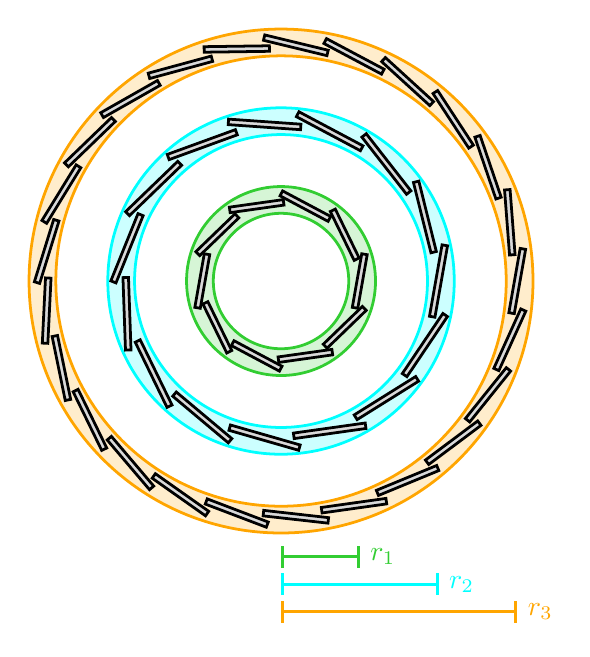
\begin{tikzpicture}[scale=0.5,line width=1pt]

    % \def\n{20}
    \def\d{4pt}

    \foreach \r/\n/\c [count=\j] in {2/10/LimeGreen, 4/15/Cyan, 6/25/Orange} {
      \pgfmathsetmacro{\da}{360/\n}
      \pgfmathsetmacro{\w}{2*3.14*\r / \n * 1.1}

      \def\dr{0.4}
      \fill[\c!20!white,even odd rule] (0,0) circle ({\r+\dr}) (0,0) circle ({\r-0.7*\dr});
      \draw[\c] (0,0) circle({\r+\dr}) (0,0) circle ({\r-0.7*\dr});

      % \node[above,\c] at (90:{\r+\dr}) {Layer \j, $r_\j$};

      \foreach \i in {1,...,\n} {
        \pgfmathsetmacro{\a}{\da * \i}
        \begin{scope}[rotate=\a,shift={(\r,0)}]
          \begin{scope}[rotate={90-10}]
            \draw[fill=black!15] ({-\w/2},{-\d/2}) rectangle ({\w/2},{\d/2});
          \end{scope}
        \end{scope}
      }

      % \draw[\c,line width=2pt] (0,0) circle(\r);
    }

    \draw[|-|,LimeGreen] (0, -7) --++(2,0) node[at end,right] {$r_1$};
    \draw[|-|,Cyan] (0, -7.7) --++(4,0) node[at end,right] {$r_2$};
    \draw[|-|,Orange] (0, -8.4) --++(6,0) node[at end,right] {$r_3$};

    % \foreach \r/\a [count=\i] in {2/0, 4/-30, 6/-60} {
    %   \draw[-|] (0,0) -- (\a:\r);
    %   \node at (\a:{\r+0.9}) {$r_\i$};
    % }

  \end{tikzpicture}

\end{document}